\qrchapter{https://forgottenpillar.com/rsc/en-fp-chapter24}{The future of the Fundamental Principles}


\qrchapter{https://forgottenpillar.com/rsc/es-fp-chapter24}{El futuro de los Principios Fundamentales}


We have already read the following quotation from the chapter “\textit{The Foundation of Our Faith}”. It is one of Sister White’s foresight of the great reformation that would take place among Seventh-day Adventists; this reformation would consist in giving up the Fundamental Principles. This is precisely how the new organization will be established.


Ya hemos leído la siguiente cita del capítulo “\textit{El Fundamento de Nuestra Fe}”. Es una de las previsiones de la hermana White sobre la gran reforma que tendría lugar entre los adventistas del séptimo día; esta reforma consistiría en renunciar a los Principios Fundamentales. Así es precisamente como se establecerá la nueva organización.


\egw{\textbf{The enemy of souls has sought to bring in the supposition that a great reformation was to take place among Seventh-day Adventists, and that this reformation would \underline{consist in giving up the doctrines which stand as the pillars of our faith} and engaging in a process of reorganization}. Were this reformation to take place, what would result? \textbf{The principles of truth that God in His wisdom has given to the remnant church would be discarded. Our religion would be changed. \underline{The fundamental principles that have sustained the work for the last fifty years would be accounted as error}}. \textbf{A new organization would be established. Books of a new order would be written. A system of intellectual philosophy would be introduced}. The founders of this system would go into the cities and do a wonderful work. The Sabbath, of course, would be lightly regarded, as also the God who created it. Nothing would be allowed to stand in the way of the new movement. The leaders would teach that virtue is better than vice; but \textbf{God being removed}, they would \textbf{place their dependence on human power}, which, without God, is worthless. Their foundation would be built on the sand, and storm and tempest would sweep away the structure.}[Lt242-1903.13; 1903][https://egwwritings.org/read?panels=p7767.20]


\egw{\textbf{El enemigo de las almas ha tratado de introducir la suposición de que una gran reforma iba a tener lugar entre los Adventistas del Séptimo Día, y que esta reforma \underline{consistiría en renunciar a las doctrinas que se mantienen como pilares de nuestra fe} y en emprender un proceso de reorganización}. Si esta reforma tuviera lugar, ¿qué resultaría? \textbf{Los principios de la verdad que Dios, en su sabiduría, ha dado a la iglesia remanente serían descartados. Nuestra religión cambiaría. \underline{Los principios fundamentales que han sostenido la obra durante los últimos cincuenta años serían considerados como un error}}. \textbf{Se establecería una nueva organización. Se escribirían libros de un nuevo orden. Se introduciría un sistema de filosofía intelectual}. Los fundadores de este sistema irían a las ciudades y harían una obra maravillosa. El sábado, por supuesto, sería considerado a la ligera, así como el Dios que lo creó. No se permitiría que nada se interpusiera en el camino del nuevo movimiento. Los líderes enseñarían que la virtud es mejor que el vicio; pero \textbf{al ser eliminado Dios}, ellos \textbf{pondrían su dependencia en el poder humano}, el cual, sin Dios, no tiene valor. Sus cimientos estarían construidos sobre la arena, y la tormenta y la tempestad barrería la estructura.}[Lt242-1903.13; 1903][https://egwwritings.org/read?panels=p7767.20]


\egwnogap{Who has authority to begin such a movement? \textbf{We have our Bibles. We have our experience, attested to by the miraculous working of the Holy Spirit}. \textbf{We have a truth that admits of no compromise.} \textbf{\underline{Shall we not repudiate everything that is not in harmony with this truth}?}}[Lt242-1903.14; 1903][https://egwwritings.org/read?panels=p7767.21]


\egwnogap{¿Quién tiene autoridad para iniciar tal movimiento? \textbf{Tenemos nuestras Biblias. Tenemos nuestra experiencia, atestiguada por la obra milagrosa del Espíritu Santo}. \textbf{Tenemos una verdad que no admite concesiones.} \textbf{\underline{¿No debemos repudiar todo lo que no esté en armonía con esta verdad}?}}[Lt242-1903.14; 1903][https://egwwritings.org/read?panels=p7767.21]


Ellen White saw the effort of the enemy to remove these \emcap{Fundamental Principles}. They have sustained the work from the beginning. They were truths attested by the miraculous working of the Holy Spirit, and they admit no compromise. \egwinline{Shall we not repudiate everything that is not in harmony with this truth?}


Elena G. de White vio el esfuerzo del enemigo por eliminar estos \emcap{Principios Fundamentales}. Ellos han sostenido la obra desde el principio. Eran verdades atestiguadas por la obra milagrosa del Espíritu Santo, y no admiten concesiones. \egwinline{¿No hemos de repudiar todo lo que no esté en armonía con esta verdad?}


\begin{figure}
    \centering
    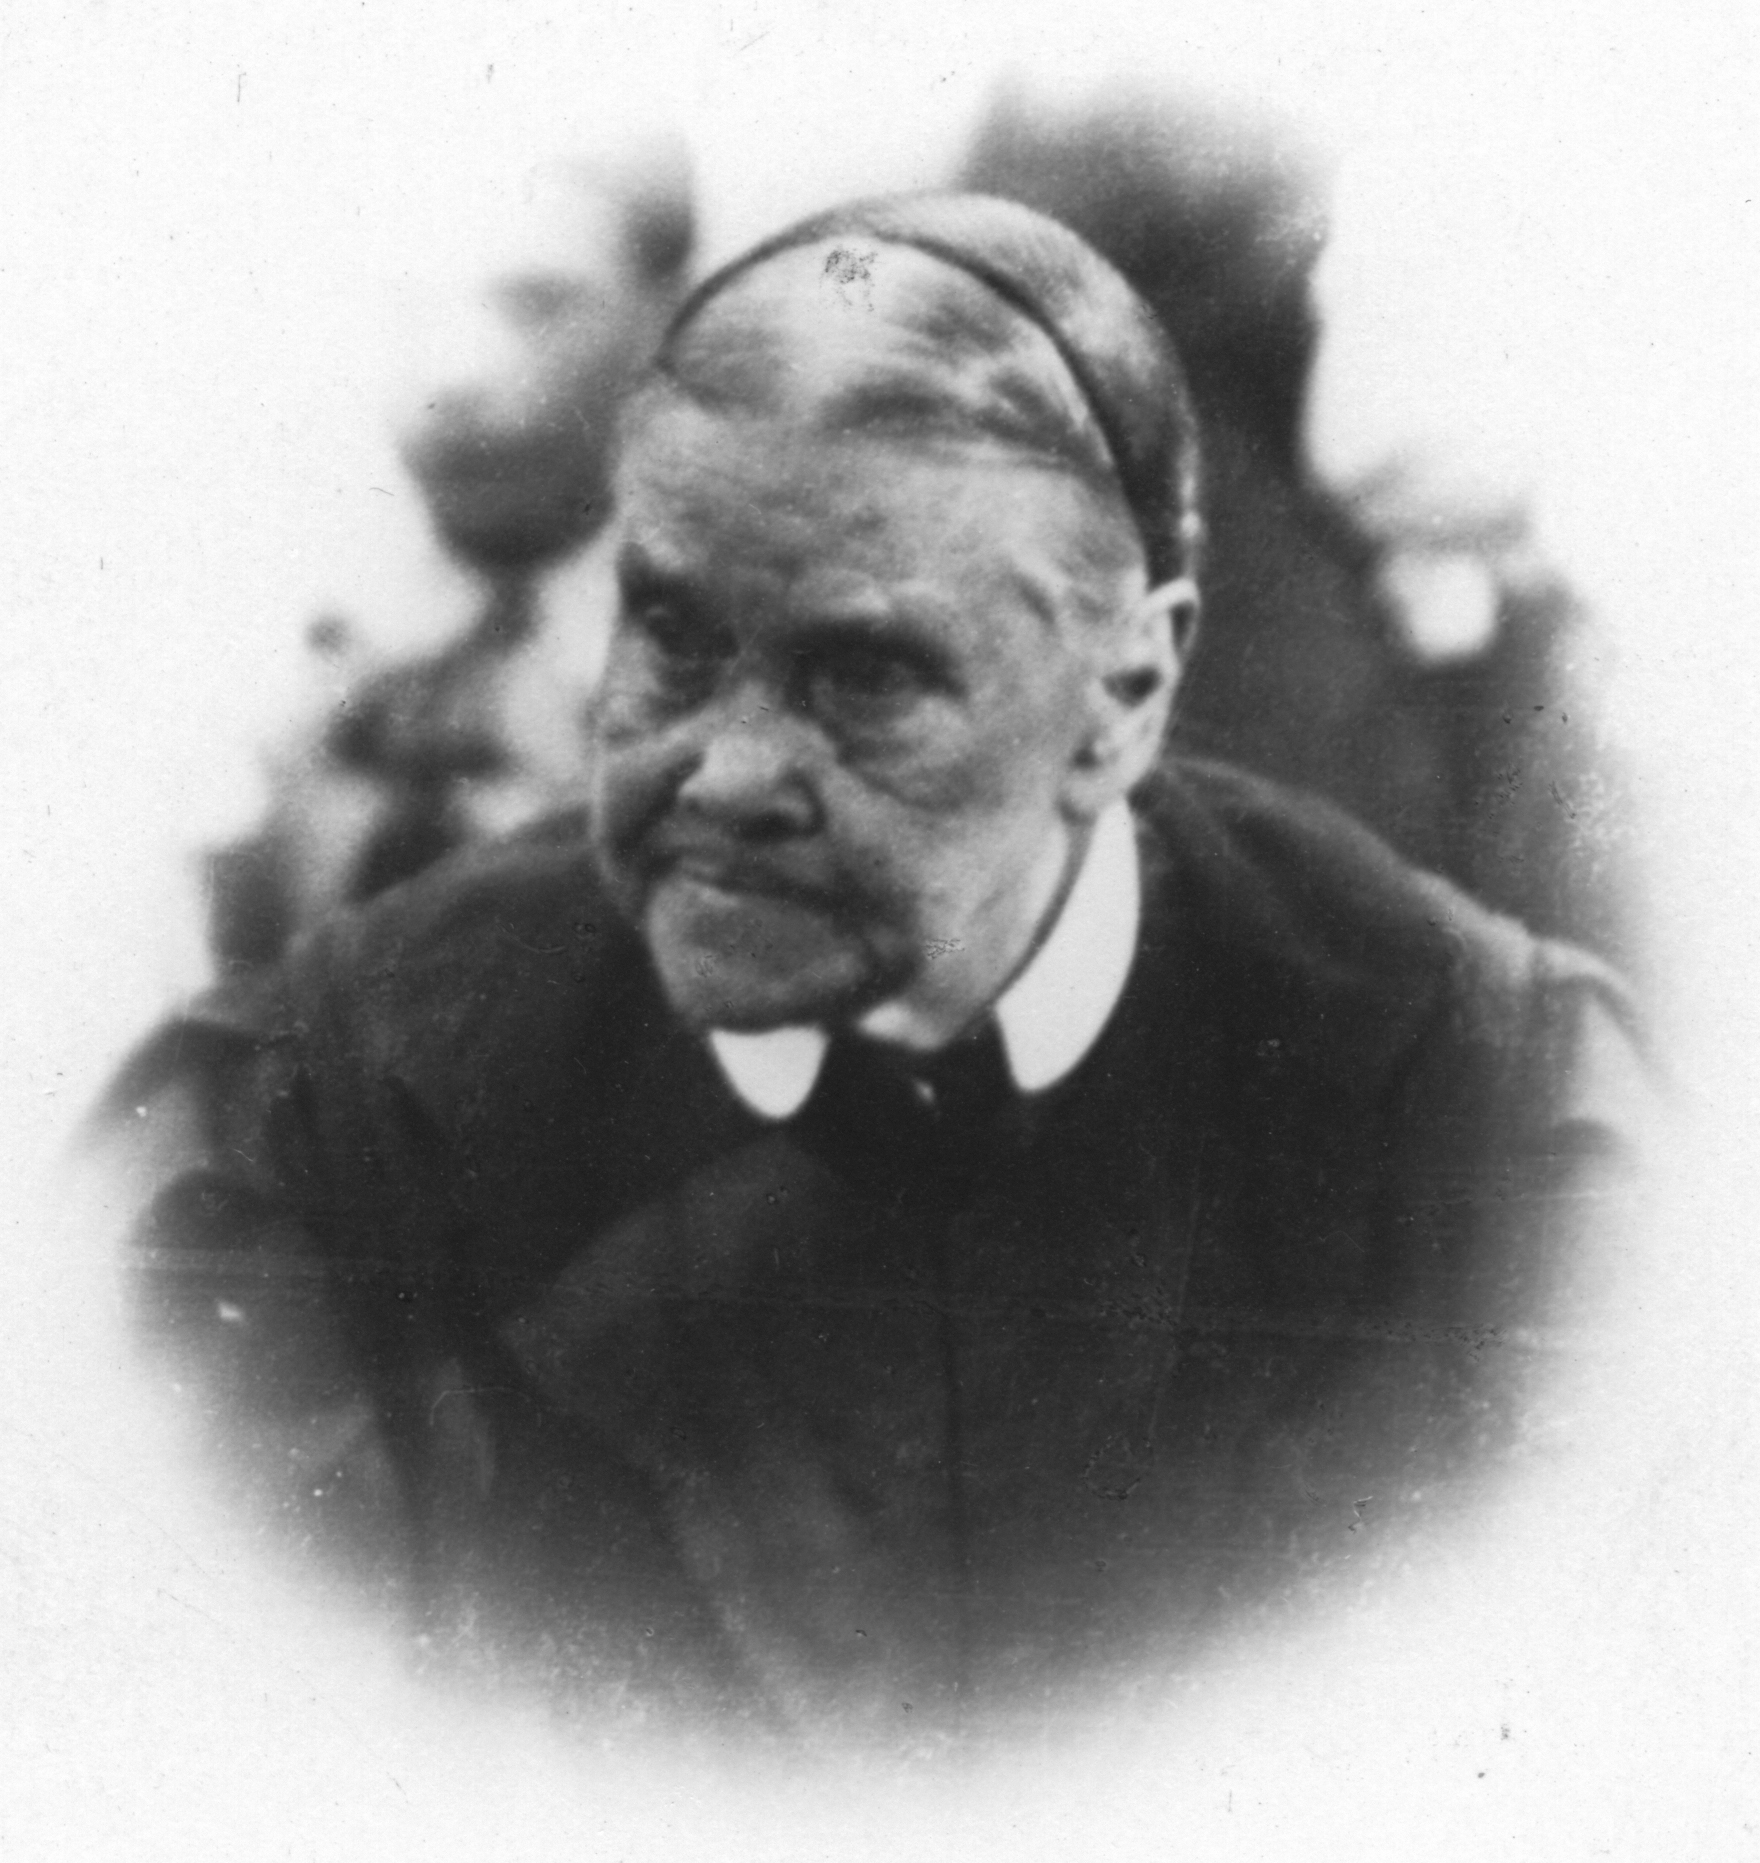
\includegraphics[width=1\linewidth]{images/ellen-white-1913.jpg}
    \caption*{Ellen G. White, 1913}
    \label{fig:e-white-1913}
\end{figure}


\begin{figure}
    \centering
    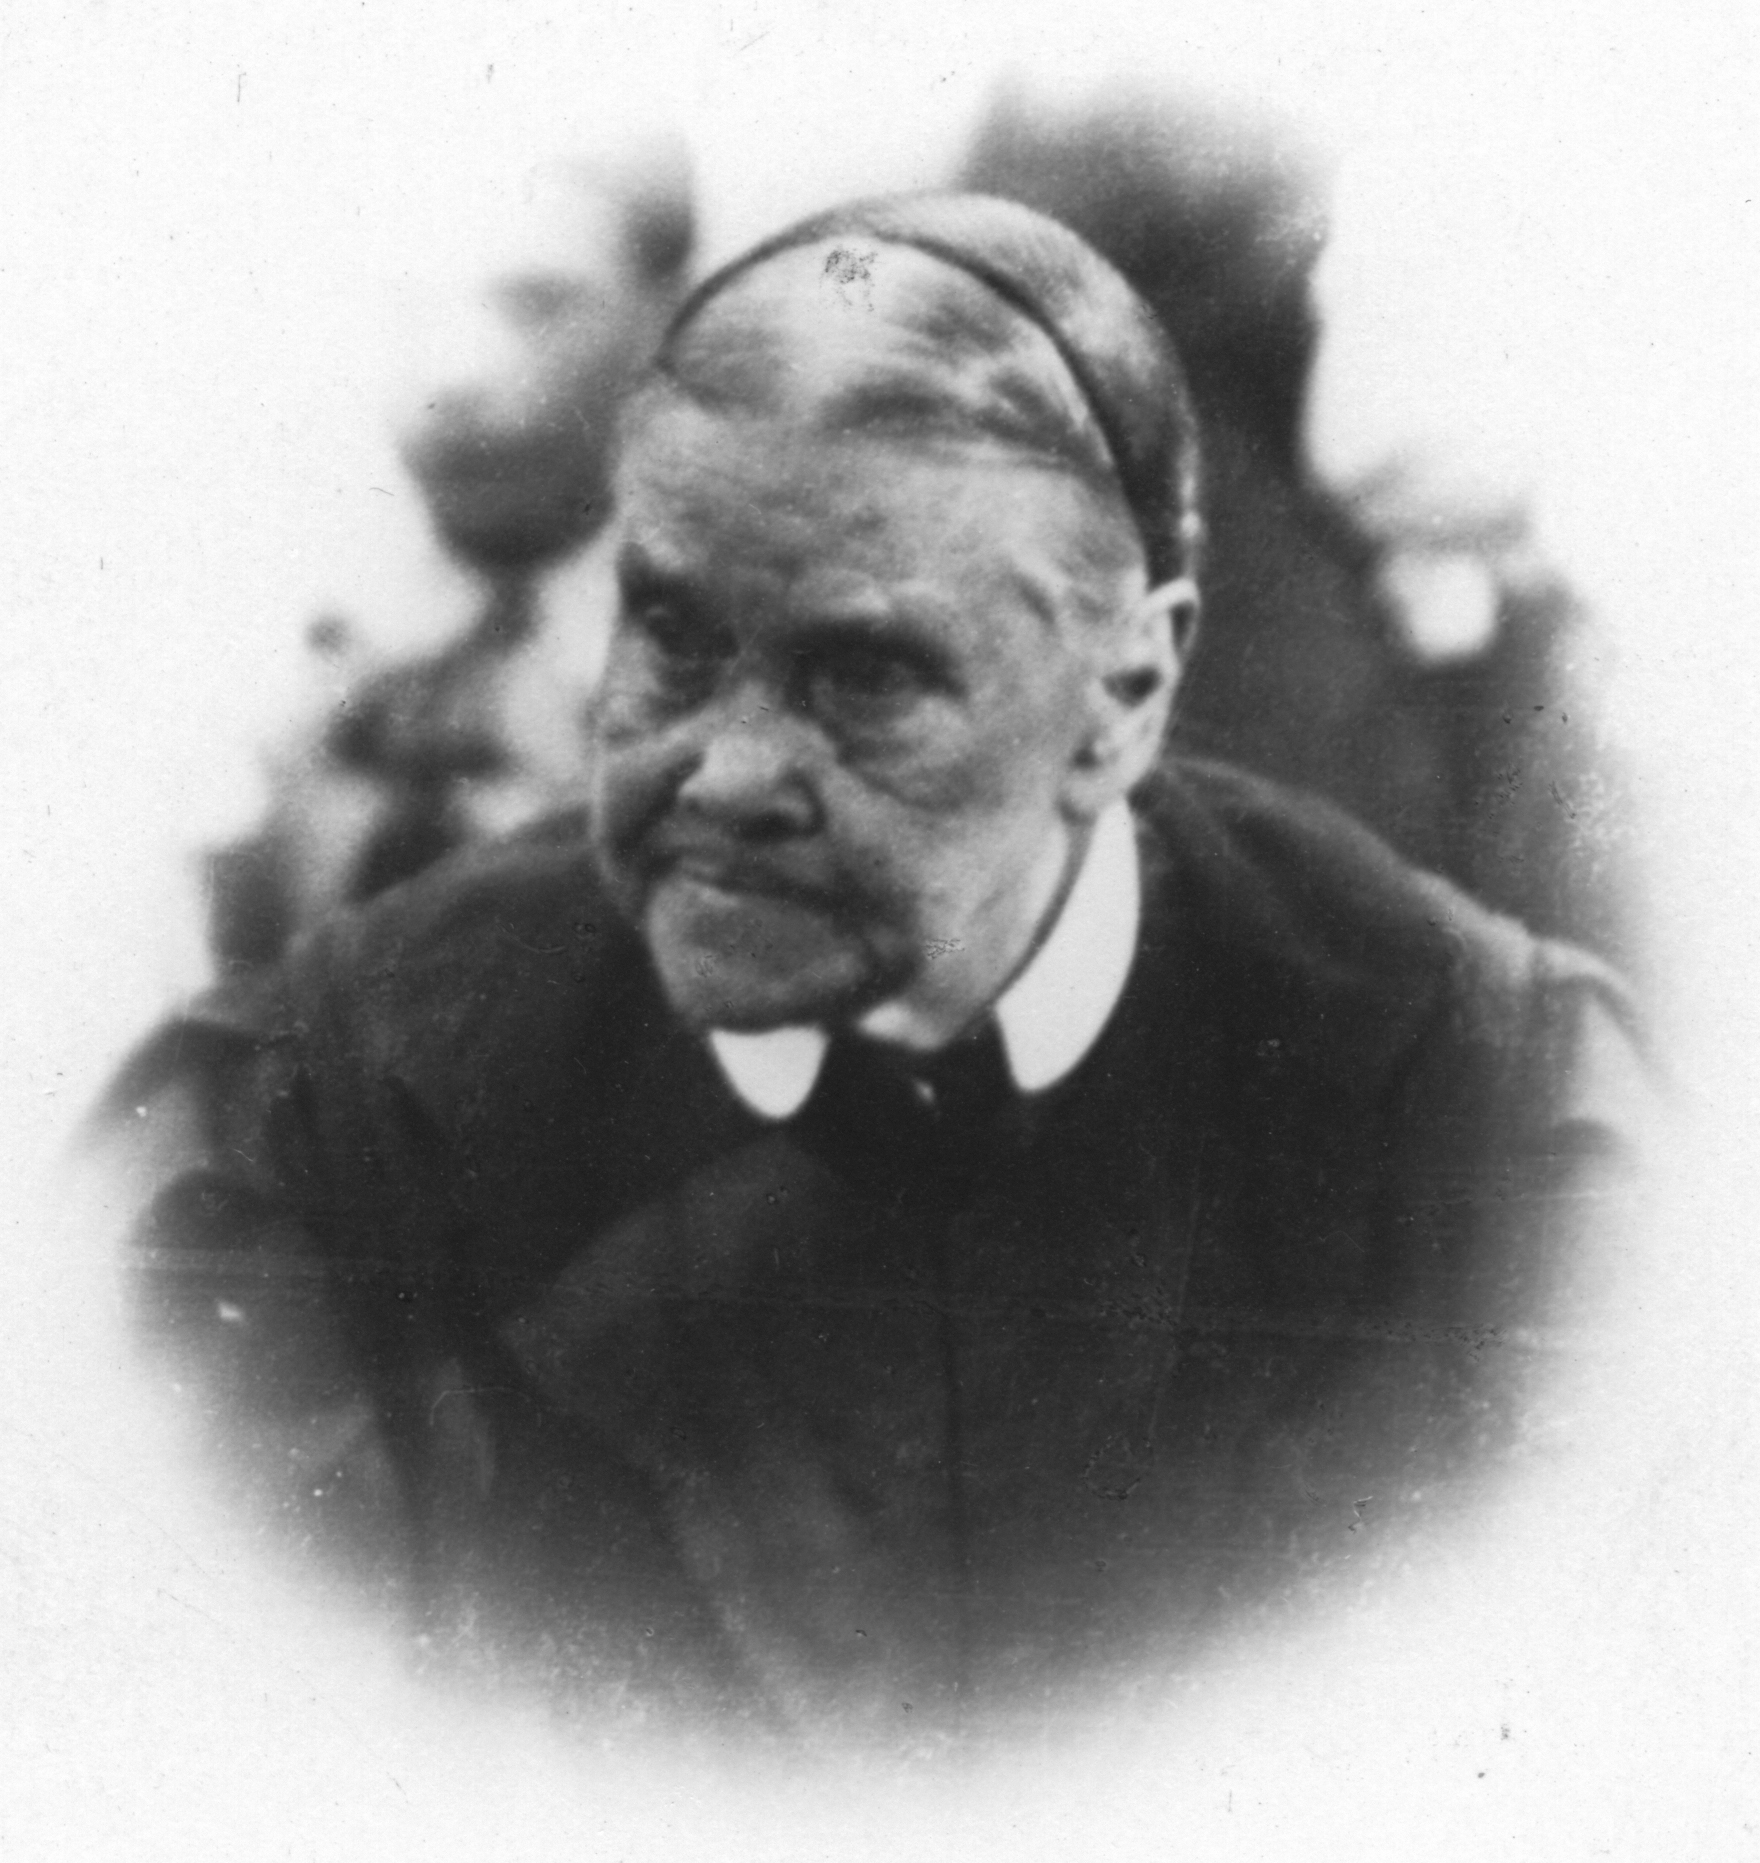
\includegraphics[width=1\linewidth]{images/ellen-white-1913.jpg}
    \caption*{Elena G. de White, 1913}
    \label{fig:e-white-1913}
\end{figure}


Sister White foretold us the future. We watch its fulfilment today. Comparing the \emcap{Fundamental Principles} with today’s Fundamental Beliefs, we see that our religion has changed. Our belief regarding the \emcap{personality of God} has changed. Books of a new order have been written, which are not based on the solid Word of God. A system of intellectual philosophy has been introduced.


La hermana White nos predijo el futuro. Hoy vemos su cumplimiento. Comparando los \emcap{Principios Fundamentales} con las creencias fundamentales de hoy, vemos que nuestra religión ha cambiado. Nuestra creencia respecto a la \emcap{personalidad de Dios} ha cambiado. Se han escrito libros de un nuevo orden, que no se basan en la sólida Palabra de Dios. Se ha introducido un sistema de filosofía intelectual.


This reformation took place in her time. This is how she described the days of the Seventh-day Adventist Church in her time and in the future:


Esta reforma tuvo lugar en su tiempo. Así es como ella describió los días de la Iglesia Adventista del Séptimo Día en su tiempo y en el futuro:


\egw{The present is a solemn, fearful time for the church. The angels are already girded, awaiting the mandate of God to pour their vials of wrath upon the world. Destroying angels are taking up the work of vengeance, for the Spirit of God is gradually withdrawing from the world. Satan is also mustering his forces of evil, going forth ‘unto the kings of the earth and of the whole world,’ to gather them under his banner, to be trained for ‘the battle of that great day of God Almighty.’ \textbf{Satan is to make most powerful efforts for the mastery in the last great conflict. \underline{Fundamental principles will be brought out, and decisions made in regard to them}. Skepticism is prevailing everywhere}. Ungodliness abounds. \textbf{The faith of individual members of the church will be tested as though there were not another person in the world}...}[Ms1a-1890.8; 1890][https://egwwritings.org/read?panels=p6780.13]


\egw{El presente es un tiempo solemne y temible para la iglesia. Los ángeles ya están ceñidos, esperando el mandato de Dios para derramar sus copas de ira sobre el mundo. Los ángeles destructores están emprendiendo la obra de la venganza, pues el Espíritu de Dios se está retirando gradualmente del mundo. Satanás también está reuniendo sus fuerzas del mal, saliendo ‘a los reyes de la tierra y del mundo entero’, para reunirlos bajo su bandera, a fin de entrenarlos para ‘la batalla de aquel gran día de Dios Todopoderoso’. \textbf{Satanás se esforzará poderosamente por dominar el último gran conflicto. \underline{Se pondrán de manifiesto los principios fundamentales y se tomarán decisiones al respecto}. El escepticismo prevalece en todas partes}. La impiedad abunda. \textbf{La fe de los miembros individuales de la iglesia será probada como si no hubiera otra persona en el mundo}...}[Ms1a-1890.8; 1890][https://egwwritings.org/read?panels=p6780.13]


Satan's most powerful efforts are to remove the \emcap{Fundamental Principles} by veiling them in skepticism. Judging from today’s perspective we testify to the truthfulness of Ellen White’s prophecies.


Los esfuerzos más poderosos de Satanás consisten en eliminar los \emcap{Principios Fundamentales} velándolos en el escepticismo. Juzgando desde la perspectiva de hoy, damos testimonio de la veracidad de las profecías de Elena G. de White.


\egw{I tell you now, that when I am laid to rest, \textbf{great changes will take place}.}[Ms1-1915.2; 1915][https://egwwritings.org/read?panels=p10771.9]


\egw{Te digo ahora, que cuando sea puesta a descansar, \textbf{ocurrirán grandes cambios}.}[Ms1-1915.2; 1915][https://egwwritings.org/read?panels=p10771.9]


The true question we have for ourselves is, when the \emcap{Fundamental Principles} are being brought out, what decision will I make in regard to them? Shall we not repudiate everything that is not in harmony with these principles? What decision will you make?


La verdadera pregunta que nos hacemos es, cuando los \emcap{Principios Fundamentales} salgan a la luz, ¿qué decisión tomaré con respecto a ellos? ¿No repudiaremos todo lo que no esté en armonía con estos principios? ¿Qué decisión tomarás tú?


% The future of the Fundamental Principles

\begin{titledpoem}
    \stanza{
        In the early whisper of prophecy’s sound, \\
        Ellen White warned where dangers abound. \\
        "The enemy plots," she sternly declared, \\
        "To dismantle truths our forebears shared."
    }

    \stanza{
        Fundamental Principles, strong and sure, \\
        Once the bedrock, pure and unpure. \\
        Now the sands shift beneath our creed, \\
        Where new doctrines grow like wayward weed.
    }

    \stanza{
        Reformation masked as light so bright, \\
        Undermines the pillars, eroding right. \\
        Books rewritten, philosophies anew, \\
        Skepticism veils what once we knew.
    }

    \stanza{
        Shall the Sabbath lose its sacred glow? \\
        Shall we forget the God that we owe? \\
        "The foundation crumbles," so it seems, \\
        As truth is lost to intellectual dreams.
    }

    \stanza{
        Look back to the days, to the Spirit-led start, \\
        Where divine truths were etched in heart. \\
        Satan’s strategies, cunning and keen— \\
        Eroding what once was clearly seen.
    }

    \stanza{
        So, brethren, now to the past return, \\
        To the roots of faith, let our hearts yearn. \\
        For the warnings spoken, the visions seen, \\
        Call us to defend what they truly mean.
    }

    \stanza{
        Stand firm in the storm as the tempests roar, \\
        Reclaim the truths worth fighting for. \\
        Ellen’s voice echoes, stark and clear: \\
        "Repudiate the false, hold the righteous near."
    }

    \stanza{
        Make your choice, as the battle lines draw, \\
        On the side of the timeless, divine law. \\
        To the Fundamental Principles, fiercely hold, \\
        The original faith, courageous and bold.
    }
\end{titledpoem}


% \qrchapter{https://forgottenpillar.com/rsc/pl-fp-chapter24}{Przyszłość Fundamentalnych Zasad}

Przeczytaliśmy już następujący cytat z rozdziału “\textit{Fundament Naszej Wiary}”. Jest to jedno z przewidywań Siostry White dotyczące wielkiej reformacji, która miała nastąpić wśród Adwentystów Dnia Siódmego; ta reformacja polegałaby na porzuceniu Fundamentalnych Zasad. Dokładnie w ten sposób zostanie ustanowiona nowa organizacja.

\egw{\textbf{Wróg dusz będzie starał się wprowadzić przypuszczenie, że wśród Adwentystów Dnia Siódmego miała nastąpić wielka reformacja, i że ta reformacja \underline{polegałaby na porzuceniu doktryn, które stoją jako filary naszej wiary} i zaangażowaniu się w proces reorganizacji}. Gdyby ta reformacja miała miejsce, co by z tego wynikło? \textbf{Zasady prawdy, które Bóg w swojej mądrości dał Kościołowi Ostatków, zostałyby odrzucone. Nasza religia zostałaby zmieniona. \underline{Fundamentalne zasady, które podtrzymywały dzieło przez ostatnie pięćdziesiąt lat, zostałyby uznane za błąd}}. \textbf{Zostałaby ustanowiona nowa organizacja. Zostałyby napisane książki nowego porządku. Zostałby wprowadzony system filozofii intelektualnej}. Założyciele tego systemu poszliby do miast i wykonaliby wspaniałą pracę. Szabat, oczywiście, byłby lekceważony, podobnie jak Bóg, który go stworzył. Nic nie mogłoby stanąć na drodze nowego ruchu. Przywódcy nauczaliby, że cnota jest lepsza od występku; ale \textbf{gdy Bóg zostałby usunięty}, \textbf{pokładaliby swoją ufność w ludzkiej mocy}, która bez Boga jest bezwartościowa. Ich fundament byłby zbudowany na piasku, a burza i nawałnica zmiotłyby tę konstrukcję.}[Lt242-1903.13; 1903][https://egwwritings.org/?ref=en\_Lt242-1903.13&para=7767.20]

\egwnogap{Kto ma autorytet, aby rozpocząć taki ruch? \textbf{Mamy nasze Biblie. Mamy nasze doświadczenie, potwierdzone cudownym działaniem Ducha Świętego}. \textbf{Mamy prawdę, która nie dopuszcza żadnego kompromisu.} \textbf{\underline{Czy nie powinniśmy odrzucić wszystkiego, co nie jest w harmonii z tą prawdą}?}}[Lt242-1903.14; 1903][https://egwwritings.org/?ref=en\_Lt242-1903.14&para=7767.21]

Ellen White widziała wysiłek wroga, aby usunąć te \emcap{Fundamentalne Zasady}. Podtrzymywały one dzieło od samego początku. Były to prawdy potwierdzone cudownym działaniem Ducha Świętego i nie dopuszczają one żadnego kompromisu. \egwinline{Czy nie powinniśmy odrzucić wszystkiego, co nie jest w harmonii z tą prawdą?}

\begin{figure}
    \centering
    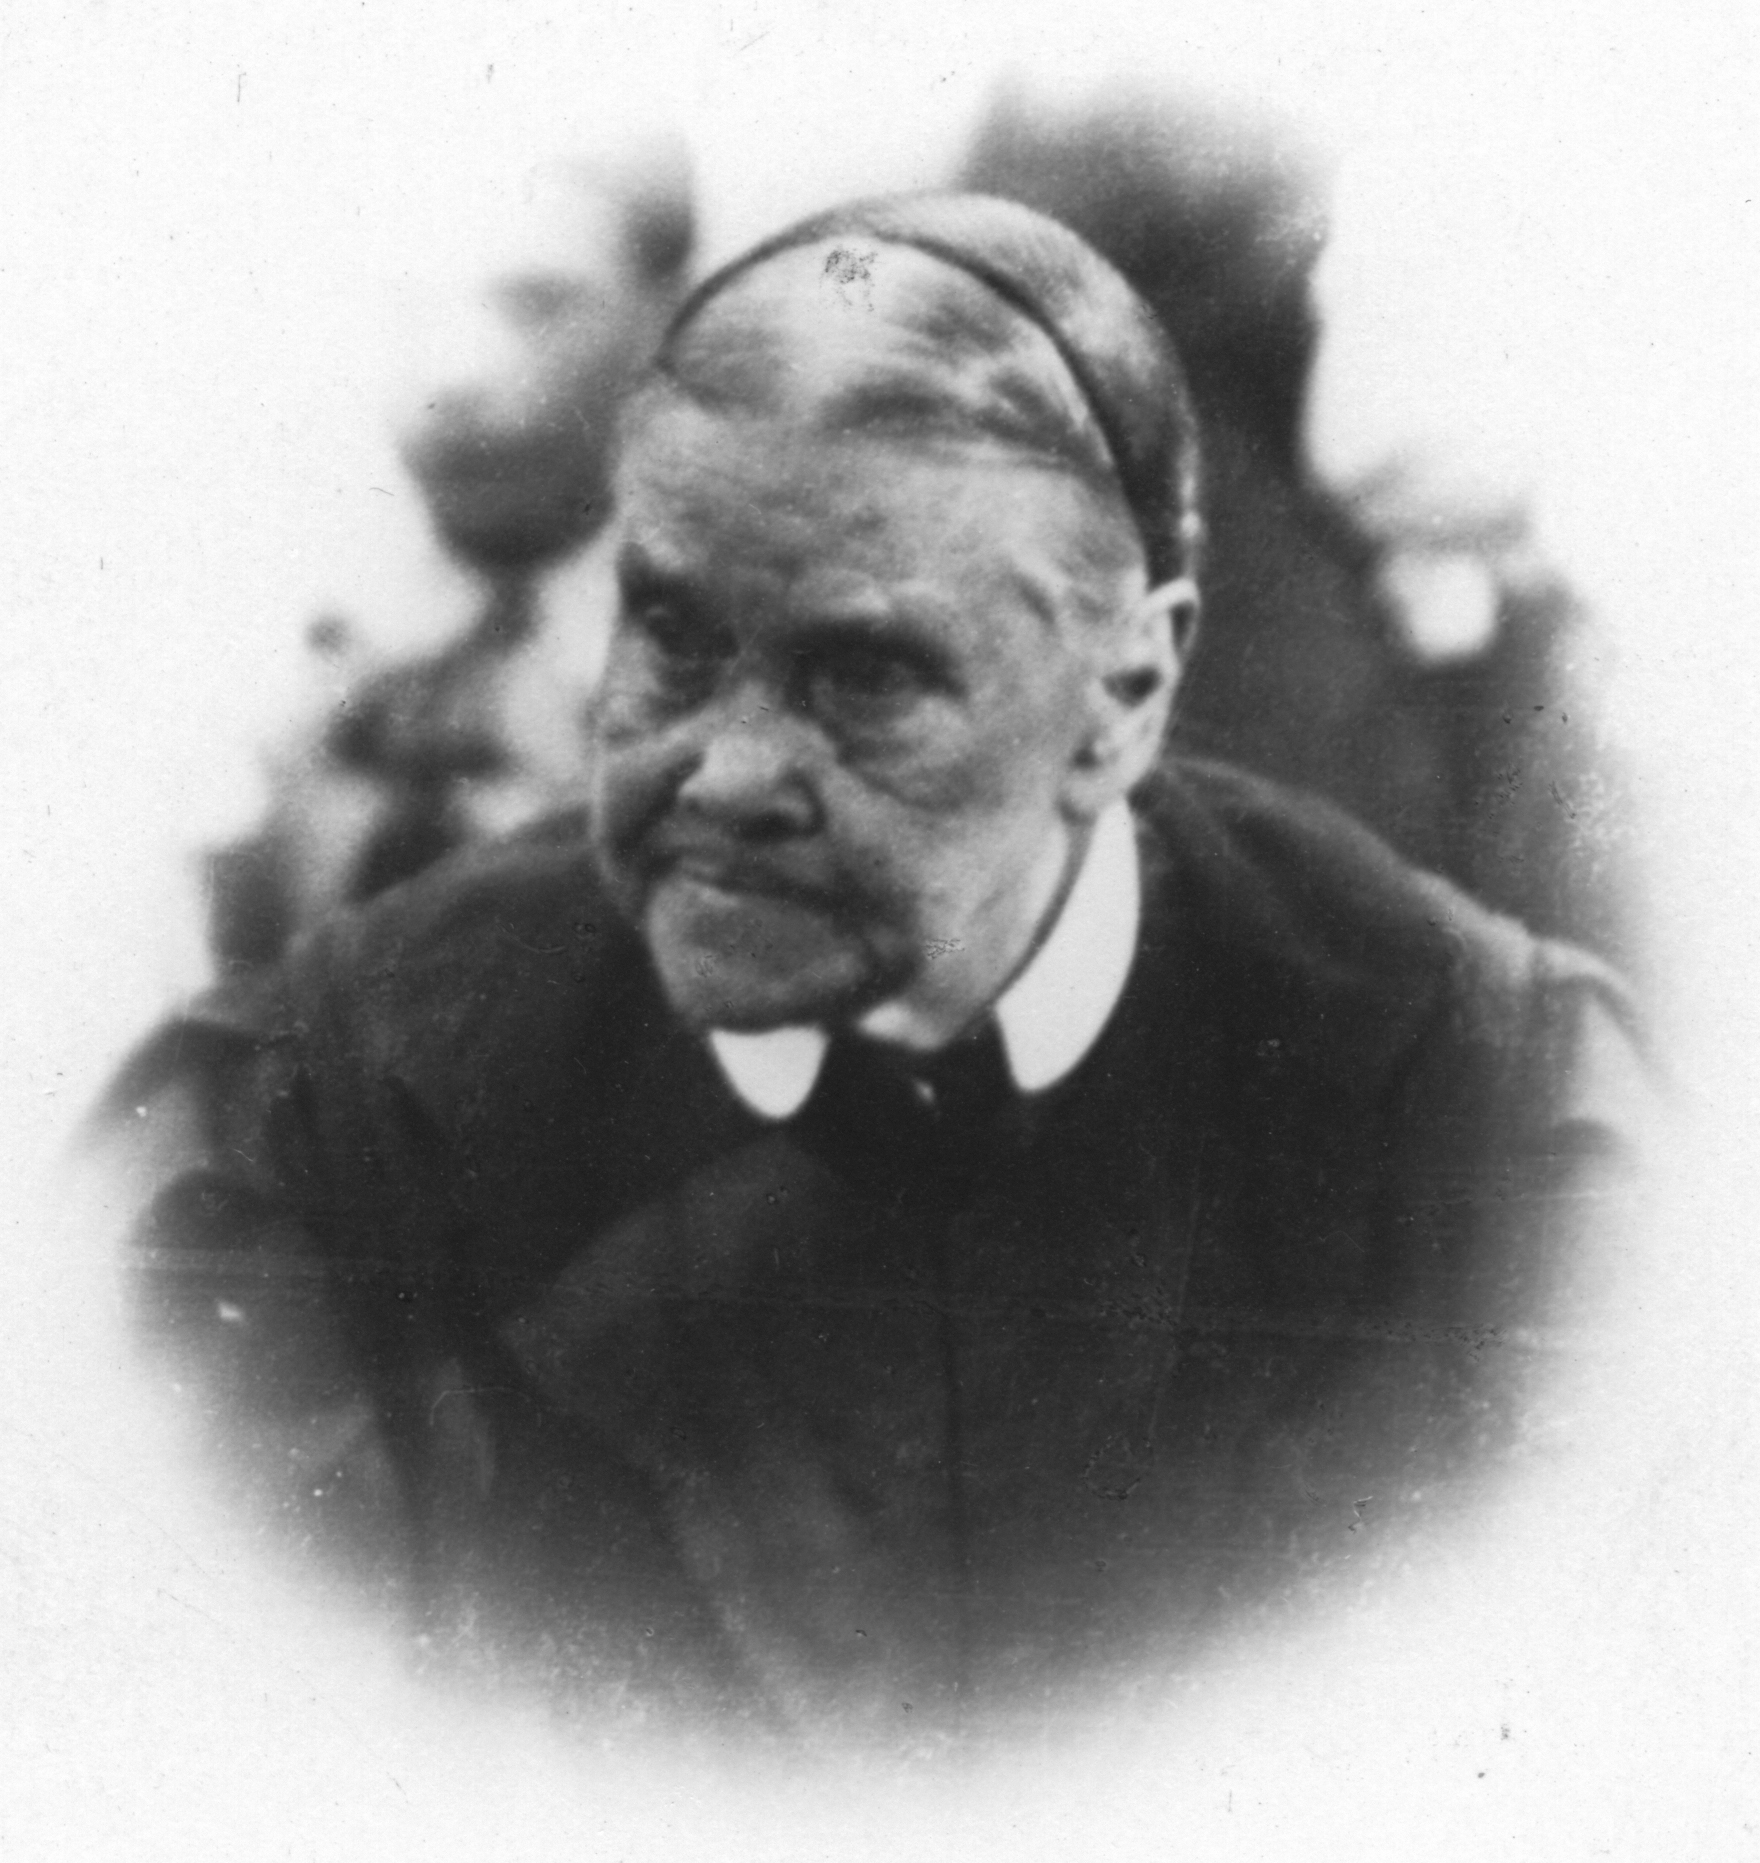
\includegraphics[width=1\linewidth]{images/ellen-white-1913.jpg}
    \caption*{Ellen G. White, 1913}
    \label{fig:e-white-1913}
\end{figure}

Siostra White przepowiedziała nam przyszłość. Dziś obserwujemy jej spełnienie. Porównując \emcap{Fundamentalne Zasady} z dzisiejszymi Fundamentalnymi Wierzeniami, widzimy, że nasza religia się zmieniła. Nasze przekonanie dotyczące \emcap{osobowości Boga} się zmieniło. Zostały napisane książki nowego porządku, które nie są oparte na solidnym Słowie Bożym. Został wprowadzony system filozofii intelektualnej.

Ta reformacja miała miejsce w jej czasach. Tak opisała dni Kościoła Adwentystów Dnia Siódmego w jej czasach i w przyszłości:

\egw{Obecny czas jest poważnym, pełnym trwogi czasem dla kościoła. Aniołowie są już przepasani, oczekując na rozkaz Boga, aby wylać swoje czasze gniewu na świat. Aniołowie zniszczenia podejmują dzieło zemsty, ponieważ Duch Boży stopniowo wycofuje się ze świata. Szatan również gromadzi swoje siły zła, wychodząc ‘do królów ziemi i całego świata’, aby zgromadzić ich pod swoim sztandarem, i przygotować do ‘bitwy w ów wielki dzień Boga Wszechmogącego.’ \textbf{Szatan podejmie najpotężniejsze wysiłki, aby zdobyć panowanie w ostatnim wielkim konflikcie. \underline{Fundamentalne zasady zostaną wydobyte na światło dzienne i zostaną podjęte decyzje w odniesieniu do nich}. Sceptycyzm przeważa wszędzie}. Bezbożność obfituje. \textbf{Wiara poszczególnych członków kościoła będzie poddana próbie, jakby nie było innej osoby na świecie}...}[Ms1a-1890.8; 1890][https://egwwritings.org/?ref=en\_Ms1a-1890.8&para=6780.13]

Najpotężniejsze wysiłki Szatana mają na celu usunięcie \emcap{Fundamentalnych Zasad} poprzez zasłonięcie ich sceptycyzmem. Oceniając z dzisiejszej perspektywy, poświadczamy prawdziwość proroctw Ellen White.

\egw{Mówię wam teraz, że kiedy zostanę złożona do grobu, \textbf{nastąpią wielkie zmiany}.}[Ms1-1915.2; 1915][https://egwwritings.org/?ref=en\_Ms1-1915.2&para=10771.9]

Prawdziwym pytaniem, które musimy sobie zadać  jest to: gdy \emcap{Fundamentalne Zasady} zostaną przedstawione, jaką decyzję podejmę w odniesieniu do nich? Czy nie powinniśmy odrzucić wszystkiego, co nie jest zgodne z tymi zasadami? Jaką decyzję podejmiesz?

\begin{titledpoem}

    \stanza{
        Proroctwa wczesny jeszcze głos \\
        Przewidział, jaki będzie los. \\
        „Diabeł ma spisek nam przeciwny, \\
        By wykraść prawdy w sposób dziwny”.
    }

    \stanza{
        Zasady, które niegdyś były, \\
        Które od Boga pochodziły, \\
        Na piasku teraz się ruszają, \\
        Bo ludzie Boga nie słuchają.
    }

    \stanza{
        Idee przebrane za światło, \\
        Usunąć filary tak łatwo. \\
        Książki też były przepisane, \\
        Nowe teorie nauczane.
    }

    \stanza{
        Czy szabat też mamy porzucić \\
        I tak od Boga się odwrócić? \\
        „Podstawy runą” — tak się zdaje, \\
        Gdy duma w miejsce prawdy staje.
    }

    \stanza{
        Wspomnijcie, jak żeśmy zaczęli, \\
        Gdy żeśmy prawdę w sercach mieli. \\
        Lecz poprzez podstępy szatana \\
        Teraz już prawda jest niechciana.
    }

    \stanza{
        Powróćmy zatem do przeszłości, \\
        Do wczesnej wiary i wierności, \\
        Bo miał zapewnić głos proroczy, \\
        Że z dobrej ścieżki nikt nie zboczy.
    }

    \stanza{
        Przetrwajmy burzę, która trwa, \\
        Gdyż warta tego prawda ta. \\
        Głosowi Ellen więc uwierzmy \\
        I prawdę drogą tak wybierzmy.
    }

    \stanza{
        A zanim przyjdzie na świat trwoga, \\
        Ustawmy się po stronie Boga. \\
        Ze starych ścieżek nie zbaczajmy \\
        I zepchnąć z nich się już nie dajmy.
    }

\end{titledpoem}

